\documentclass[12pt]{article}
\usepackage{sbc-template}
\usepackage{graphicx,url}
\usepackage{booktabs}
\usepackage[utf8]{inputenc}
\usepackage[brazil,english]{babel}

% Falta acertar referências sugeridas pelo Schnorr %

\sloppy
\title{Experimental Validation of SimGrid Predictions for RTM Applications in Multi-Node Multi-GPU Environments}
\author{Arthur Andrade da Silva\inst{1}, Vin{\'i}cius Daniel Spadotto\inst{1}, Cristiano Alex Künas\inst{1},\\
Lucas Mello Schnorr\inst{1}, Phillipe Olivier Alexandre Navaux\inst{1}}
\address{Institute of Informatics, Federal University of Rio Grande do Sul (UFRGS)\\
Caixa Postal 15.064 -- 91.501-970 -- Porto Alegre -- RS -- Brazil\\
\email{\{aasilva, vinicius.spadotto, cakunas, schnorr, navaux\}@inf.ufrgs.br}}
\begin{document} 
\maketitle

\begin{abstract}
Simulation models calibrated on one hardware generation are reused to predict performance on different platforms, without the cost of that extrapolation being known. This work determines the validity envelope of one such prediction. The SimGrid/SMPI model of Fletcher, an anisotropic reverse time migration (RTM) application, was calibrated with one GPU per node and a 1~Gbit/s network, and projected that higher bandwidths would increase the fraction of time spent computing, a prediction never confronted with multi-node, multi-GPU hardware. We run Fletcher's CUDA backend on the \textit{chuc} cluster of Grid'5000, with four A100 GPUs per node, across one to four nodes and bandwidths of 1, 10, and 25~Gbit/s, in order to identify under which conditions the prediction remains usable. The predicted trend holds qualitatively, but its quantitative validity diverges with scale. The spread in effective overlap across bandwidths grows from 1.3 to 38.2 percentage points between one and four nodes, and the return above 10~Gbit/s is limited. The direction of the effect extrapolates; its magnitude requires measurement.
\end{abstract}

\section{Introduction}
Reverse time migration (RTM) produces subsurface images from seismic data recorded at the surface and is the reference method in oil and gas exploration. Its computational cost places it among the recurring workloads in high-performance computing, which motivated GPU-accelerated implementations since the first ports of the finite-difference kernel to CUDA \cite{micikevicius2009fd3d}. Among them is Fletcher, which solves wave propagation in anisotropic media with a tilted symmetry axis by finite differences over a regular 3D grid, with backends for CPU and GPU.

In distributed memory, this grid is partitioned across processes, and the stencil requires at each time step the values in the neighborhood of every point. Implementations may satisfy this requirement in different ways; the one evaluated in this work exchanges ghost cells between adjacent subdomains via the Message Passing Interface (MPI) \cite{spadotto2026sbacpad}. The decomposition strategy fixes the ratio between communication surface and computational volume, hence how much of the exchange can be hidden under computation. GPU acceleration unbalances the two terms. Time per step decreases with computational throughput while the exchanged volume stays the same, leaving less computation to mask communication, and on platforms with multiple accelerators per node it is inter-node communication that constrains scalability.

Fletcher's other limiting factors have already been characterized experimentally. \cite{rigon2024otimizando} overlapped point-to-point communication among GPUs within a node with grid computation, reducing the energy-delay product by up to 40\%, and \cite{kunas2024enhancing} overlapped input/output (I/O) checkpoints with computation, later evaluating compression to reduce I/O volume \cite{kunas2025compressao}. Communication across multiple nodes remains without direct measurement at the bandwidths of current hardware. The prior study of this implementation validated inter-node communication up to 10~Gbit/s on CPU only, and up to 1~Gbit/s with GPU \cite{spadotto2026sbacpad}. Beyond that point the available evidence comes from simulation. A model built with SimGrid and its simulated MPI component (SMPI), calibrated on a cluster with one GPU per node and a 1~Gbit/s network, projected that higher bandwidths would raise the fraction of time devoted to computation and reduce total runtime \cite{spadotto2026carla,spadotto2026tcc}, the only prediction available on the axis this work measures.

SimGrid's validation program does not cover this scenario. It has been validated for conventional networks and, separately, for CUDA kernels on a single GPU, but multi-GPU nodes fall outside that coverage (Section~2.2), so no empirical evidence attests that a prediction calibrated on single-GPU hardware remains valid on such platforms.

The objective of this work is to determine the validity envelope of that prediction, the conditions of bandwidth and scale under which it remains usable for infrastructure dimensioning. We run Fletcher's CUDA backend across topologies from one to four nodes, under controlled bandwidth, with repetitions that quantify the variability of a shared infrastructure, confronting the measurements against the equivalent simulated predictions. The main result is that the predicted trend survives the change of hardware generation in direction but not in magnitude, with the spread in effective overlap across bandwidths growing from 1.3 percentage points at one node to 38.2 at four, a scale dependence the original model does not express. This yields the direct measurement, on multi-node, multi-GPU hardware, of the masking predicted by the model, delimiting the conditions under which the prediction holds, together with the experimental framework built to conduct it, with infrastructure validation, per-repetition structural verification of network shaping, and provenance tracking \cite{cherrueau2022enoslib}, released with this article.

Section~2 covers domain decomposition, SimGrid's validation reach, and related work. Section~3 describes the implementation and resulting hypotheses. Section~4 details the methodology. Section~5 presents results and discussion. Section~6 concludes.

\section{Background and Related Work}

Fletcher's domain decomposition determines the volume communicated per unit of computation; SimGrid's validation program delimits what has already been verified in the simulator; and the related work situates this study among earlier attempts to confront simulation with real execution.

\subsection{Fletcher and Domain Decomposition}
RTM propagates the seismic wavefield forward in time from the source and backward from the receivers. Cross-correlation between the two fields locates geological reflectors with greater precision than simplified methods \cite{zhou2018rtm}. In distributed memory, the regular 3D grid is partitioned across processes and subdomain borders are exchanged at every step.

\begin{figure}[tb]
  \centering
  \begin{minipage}{0.48\linewidth}
    \centering
    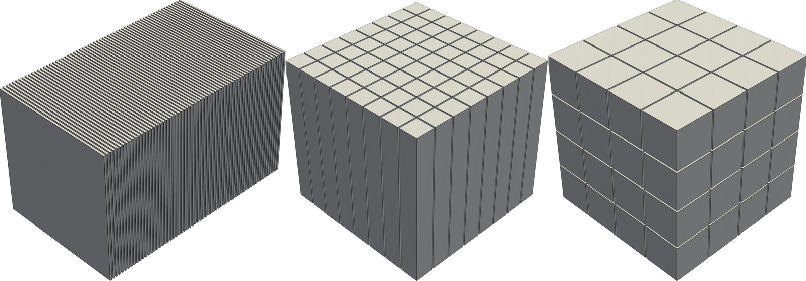
\includegraphics[width=\linewidth]{partitioning_methods.pdf}
  \end{minipage}\hfill
  \begin{minipage}{0.48\linewidth}
    \centering
    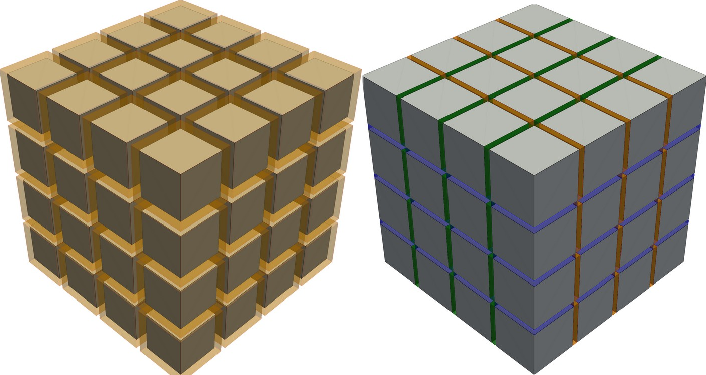
\includegraphics[width=\linewidth]{ghost_cells_cubes.pdf}
  \end{minipage}
  \caption{3D domain decomposition (left) and ghost cells under block decomposition (right). Adapted from \cite{spadotto2026tcc}.}
  \label{fig:decomp}
  \label{fig:ghostcells}
\end{figure}

Under slices (1D), each process keeps two full domain faces as communication surface, which does not shrink as the number of processes grows (Figure~\ref{fig:decomp}). Under blocks (3D), the decomposition used by \cite{pearson2020nodeaware} in a related stencil application, the surface per subdomain decreases with partitioning, at the cost of more neighbors per process. This surface-to-volume ratio is the mechanism by which node count affects performance, independently of bandwidth. The border data exchanged at each step are the ghost cells (Figure~\ref{fig:ghostcells}), whose volume depends on the wave equation formulation adopted. In the isotropic case, propagation is described by the acoustic wave equation
\begin{equation}
\frac{\partial^2 p(\vec{x},t)}{\partial t^2} = v(\vec{x})^2 \nabla^2 p(\vec{x},t),
\label{eq:acoustic}
\end{equation}
where $p(\vec{x},t)$ is pressure, $v(\vec{x})$ is velocity, and $\vec{x}=(x,y,z)$ are the spatial coordinates. Fletcher's method extends this formulation to media with a tilted symmetry axis (TTI), replacing it with a pseudo-acoustic system coupling a main pressure field and an auxiliary one, parameterized by the medium's dip and azimuth angles \cite{fletcher2009tti}, which increases the volume of borders transferred per iteration relative to the acoustic case. Asynchronous point-to-point calls hide part of that cost by exposing the domain interior to computation while borders are in flight, a pattern used since the earliest multi-GPU finite-difference implementations in CUDA \cite{micikevicius2009fd3d} and adopted in the implementation evaluated here \cite{spadotto2026sbacpad}; how much of that overlap materializes depends on the balance the simulation model attempts to predict.
\subsection{SimGrid/SMPI and the Reach of Existing Validation}
SimGrid's SMPI component \cite{casanova2014simgrid} runs unmodified MPI applications under simulated network and computation models, projecting performance on physically inaccessible platforms; that capability sustains its use in dimensioning studies and raises the question of how far its predictions can be taken. The prior Fletcher study chose SMPI because it emulates the real source code, preserving effects that coarser-grained models ignore, such as PCIe bus transfers and network contention \cite{spadotto2026carla,hoefler2010loggopsim}.

\cite{velho2013tcp} validated the flow-level network models used for TCP in \textit{Grid} and \textit{Cloud} settings; \cite{degomme2017smpi} validated SMPI for unmodified MPI applications; \cite{cornebize2021predictions} added a platform calibration methodology, with error below approximately 15\% for messages up to 1~GiB, used to calibrate the Fletcher model. Extensions have been validated on other large-scale platforms without accelerators, among them the Tibidabo ARM cluster \cite{bedaride2013tibidabo}, the BigDFT electronic-structure code \cite{degomme2017smpi}, and the StarPU task runtime \cite{stanisic2015starpu}. The simulator has also been extended to accelerators, but under a different scope. \cite{boughzala2020simgridgpu} model the energy consumption of CUDA kernels on a single GPU, without addressing inter-node communication. What remains without experimental coverage is inter-node communication on hardware with multiple GPUs per node \cite{unat2026gpucomm}, precisely the condition under which the Fletcher prediction would need to be reused on current hardware.
\subsection{Related Work}
\cite{tesser2017simulation} validated dynamic load-balancing predictions for Ondes3D, an iterative seismic finite-difference application over-decomposed in AMPI/Charm++ and structurally akin to Fletcher, against real execution on the Parapluie cluster of Grid'5000. The evaluation followed two phases, controlled validation with simulated-versus-real makespan errors between roughly 1\% and 9\%, and simulation-guided exploration of parameters whose exhaustive testing on real hardware would be prohibitive. This work adopts the same incremental-validation principle, under a distinct condition. Simulation and execution there share the same hardware generation, with no GPUs involved, whereas here the execution target differs from the one the model was calibrated on.

Within Fletcher itself, the bottlenecks already measured (Section~1) delimit what remains to be measured; none of those prior efforts \cite{rigon2024otimizando,kunas2024enhancing,kunas2025compressao} reaches inter-node communication via MPI (Table~\ref{tab:related-work}). Closest to this work, \cite{spadotto2026sbacpad} reports both simulated and real results for the multi-node MPI implementation, but with inter-node communication evaluated up to 10~Gbit/s on CPU and up to 1~Gbit/s on GPU. We found no work in the literature experimentally assessing simulation predictions for inter-node communication under a change of hardware generation; the Fletcher prediction offers a concrete case, calibrated at 1~Gbit/s with one GPU per node and restricted to that condition.

\begin{table}[tb]
  \centering
  \small
  \caption{Comparison between this work and the closest related literature.}
  \label{tab:related-work}
  \resizebox{0.99\linewidth}{!}{%
  \begin{tabular}{lccc}
    \toprule
    Work & Real hardware & Multi-GPU/node & Automated framework \\
    \midrule
    \cite{tesser2017simulation}    & Yes & No               & No  \\
    \cite{rigon2024otimizando}     & Yes & Yes (intra-node) & No  \\
    \cite{kunas2024enhancing}      & Yes & n/a              & No  \\
    \cite{kunas2025compressao}     & Yes & n/a              & No  \\
    \cite{spadotto2026sbacpad}     & Yes & Yes (multi-node only) & Yes \\
    This work                       & Yes & Yes              & Yes \\
    \bottomrule
  \end{tabular}}
\end{table}

\section{The MPI-Based Fletcher Implementation Used in This Work}

The parallel implementation and its physical evaluation at PCAD establish the calibration point, and the simulated extension of that model produces the hypotheses confronted here.

\subsection{Implementation}
The implementation evaluated here is the one built by \cite{spadotto2026sbacpad}, on which the simulation model was calibrated. It adopts a coordinator-worker MPI model, with cubic block decomposition when the process count factors evenly into three dimensions and slices otherwise, a distinction decisive for scalability (Section~3.2). Communication and computation overlap through asynchronous ghost cell exchange (Section~2.1), with backends in OpenMP for CPU and CUDA for GPU, the latter run here, in which only the ghost cell buffers cross the host-device boundary \cite{micikevicius2009fd3d,pearson2020nodeaware}. The numerical correctness of both backends was validated by \cite{spadotto2026sbacpad}.

\subsection{The Limits of the Prior Evaluation and the Resulting Hypotheses}
The physical evaluation carried out by \cite{spadotto2026sbacpad} took place at the High-Performance Computing Park (PCAD) of UFRGS, on two clusters specified in Table~\ref{tab:platform-comparison}. The CPU cluster \textit{cei} had six nodes and 10~Gbit/s links, and the GPU cluster \textit{poti}, five nodes, one NVIDIA RTX~4070 per node, and a 1~Gbit/s network. The two produced opposite behaviors. On \textit{cei}, communication was masked by computation, with computational load fractions of approximately 75\% at $256^3$ and 87\% at $512^3$; on \textit{poti}, that fraction stagnated around 20\% regardless of problem size, with the 1~Gbit/s link dominating runtime even at $512^3$, since computation there was fast enough to no longer hide communication. Verifying whether higher bandwidth would restore masking would have required an environment PCAD did not offer. The evaluation was limited to five GPUs, one per node, and both decompositions with multiple GPUs per node and networks above 1~Gbit/s remained physically inaccessible.

To reach those conditions, \cite{spadotto2026carla} calibrated a SimGrid/SMPI model following Cornebize's methodology \cite{cornebize2021predictions}, with network calibration error below approximately 15\% for messages up to 1~GiB, and used it to evaluate the application at 10 and 100~Gbit/s, plus a $\{2,2,2\}$ block decomposition with eight workers that the five-node cluster could not accommodate. Simulated computational load fractions reached approximately 65--80\% at 10~Gbit/s and, at 100~Gbit/s, 85--90\% at $256^3$ and above 90\% at $512^3$, against the 20\% measured at 1~Gbit/s. At $512^3$, the block decomposition with eight workers attained a simulated throughput of 8,309~MSamples/s at 10~Gbit/s and 9,374~MSamples/s at 100~Gbit/s, while slices with five workers remained below the single-node baseline of 3,870~MSamples/s under both conditions.


% TODO Cristiano e Arthur: deixar mais claro essa hipótese pois não fica claro o relacionamento e   ntre o que é deste trabalho deste artigo e o que é dos trabalhos anteriores [descritos nos dois parágrafos anteriores].

The two effects projected by the simulated extension of the prior study, described above, provide the hypotheses assessed experimentally in this work. The first is that masking recovers as bandwidth increases, reversing the stagnation measured at 1~Gbit/s, but saturates above 10~Gbit/s, as indicated by the mere 13\% gain from a tenfold bandwidth increase. The second is that decomposition topology weighs more than available bandwidth, since slices does not surpass single-node execution under any simulated condition. Neither hypothesis was previously tested against real execution, since the calibration infrastructure could not reproduce the required conditions, in particular multiple GPUs per node and bandwidth above 1~Gbit/s. This work performs that test on the \textit{chuc} cluster of Grid'5000.

\section{Methodology}

This section evaluates those hypotheses through real execution. Section~4.1 specifies the platform and execution framework, Section~4.2 the metrics, and Section~4.3 the threats to validity, organized in three phases of progressive departure from the calibration point.

The three phases follow the incremental validation principle of Tesser et al. (Section~2.3), quantifying fidelity first under the conditions closest to calibration. In the first, the CUDA backend runs on A100 hardware under bandwidth shaped at 1, 10, and 25~Gbit/s, at the problem sizes of the prior study's GPU range ($128^3$, $256^3$, $512^3$), under block decomposition; the four-GPUs-per-node granularity of \textit{chuc} does not accommodate a direct replica of the prior study's five-process slices configuration, so this phase concentrates on the topology that dominates the original simulated results. The 1 and 10~Gbit/s levels correspond to PCAD's physical condition and to the first simulated scenario; 25~Gbit/s, the highest point reproducible here, covers the region of diminishing returns indicated by the simulation, obviating the 100~Gbit/s point. Results are compared against the equivalent simulated predictions.

In the second phase, the same problem sizes run under the cluster's native bandwidth, a condition not evaluated in the original study; absent a simulated counterpart, results are reported descriptively, supported by the per-run decomposition of time into MPI versus CUDA. In the third, the original simulation is used in a strong scaling sweep from 1 to 16 GPUs and at a problem size beyond the original range, feasible by the A100's larger memory, with verification on real hardware at each additional node. A direct comparison between blocks and slices on real hardware is left for future work.
 
\subsection{Platform}
 
The experiments run on the \textit{chuc} cluster, at the Lille site of Grid'5000 \cite{balouek2013grid5000}, with eight nodes, each with an AMD EPYC 7513, four NVIDIA A100-SXM4-40GB GPUs, 512~GiB of RAM, and links of up to 25~Gbit/s over 2$\times$ ConnectX-5 NICs, hardware capable of GPUDirect Remote Direct Memory Access (RDMA) \cite{potluri2013gpudirect}. That capability is not exercised here. The OpenMPI/UCX stack built for this campaign was compiled \texttt{--without-cuda} and links no CUDA-aware UCX transport module, so no code path in this campaign moves MPI buffers directly from device memory, independently of what the application requests. All four GPUs of every allocated node are used in all configurations, so the node count and GPU count scale together (Table~\ref{tab:main-results}). The campaign is capped at four of the cluster's eight nodes, a limit set by allocation constraints due to queue competition on this shared, federated infrastructure.

Table~\ref{tab:platform-comparison} compares this environment against the PCAD clusters, which differ in GPU architecture, GPUs per node, interconnect, and communication path, varying jointly and not confined to device count. The calibration point uses a consumer-class GPU (RTX~4070), whereas \textit{chuc} employs datacenter-class accelerators (A100) with a distinct memory hierarchy, so the extrapolation is subject to a change of network and accelerator class simultaneously.

\begin{table}[tb]
  \centering
  \small
  \caption{Hardware environments of the prior study's physical evaluation and of this work.}
  \label{tab:platform-comparison}
  \resizebox{0.99\linewidth}{!}{%
  \begin{tabular}{lccc}
    \toprule
     & PCAD \textit{cei} (CPU) & PCAD \textit{poti} (GPU) & Grid'5000 \textit{chuc} \\
    \midrule
    Nodes & 6 & 5 & 8 \\
    Processor & 2$\times$ Xeon E5-2699, 2.0~GHz & Core i7-14700KF, 3.4~GHz & AMD EPYC 7513 (Zen~3) \\
    Cores/threads per node & 24 / 48 & 20 / 28 & 32 cores, 1 CPU/node \\
    RAM per node & 256~GB DDR4 & 96~GB DDR5 & 512~GiB \\
    GPUs per node & n/a & 1$\times$ RTX 4070 (12~GB) & 4$\times$ A100-SXM4-40GB \\
    Network & 10~Gbit/s & 1~Gbit/s & 25~Gbit/s (2$\times$ ConnectX-5) \\
    \midrule
    Used in & Prior work & Prior work & This work \\
    \bottomrule
  \end{tabular}}
\end{table}
 
An experimental framework sustains reproducibility. Before each run it validates the allocated infrastructure, including full GPU availability per node, and aborts on degraded allocation. The bandwidth of each shaping condition is imposed with \texttt{tc} (Linux Traffic Control) and a \texttt{tbf} queueing discipline, whose configuration is recorded in the metadata of every repetition, confirming that the nominal rate was applied to the interface; an independent \texttt{iperf3} probe exists but is not persisted systematically (Section~4.3). CSV-parameterized execution, checkpoint/resume, and provenance tracking complete the design, following the practice of orchestration libraries for Grid'5000 such as EnOSlib \cite{cherrueau2022enoslib}. The application source code is available online\footnote{\url{https://github.com/dannful/distributed-cube-average/}}.
 
\subsection{Metrics}
 
The primary metric is the \textbf{effective overlap ratio (ME)}, the fraction of wall-clock time per process devoted to computation rather than to blocking MPI calls; less sensitive to a change of GPU architecture than absolute throughput, it is the metric reported per topology and bandwidth in Table~\ref{tab:main-results} and Figures~\ref{fig:me-vs-nodes} and~\ref{fig:diminishing-returns}, following the line of MPI overlap quantification of \cite{denis2016overlap}, revised by \cite{medvedev2022imbasync} and used by the prior study \cite{spadotto2026carla}. The \textbf{fidelity error} takes the percentage difference between simulated prediction and real measurement under equivalent configurations. Three further measures provide context. \textbf{Throughput} and \textbf{makespan} give the absolute performance reading, comparable to the prior study's MSamples/s figures; the \textbf{structural confirmation of shaping} verifies that nominal conditions were correctly configured, without independent per-run bandwidth measurement (Section~4.1); and the \textbf{MPI-versus-CUDA time decomposition} grounds mechanistic explanations for observed divergences.
 
\subsection{Threats to Validity}
 
Hardware generation, network topology, and communication path vary jointly between calibration and test, so any observed divergence reflects their combination rather than an isolated factor; this entanglement is itself the scenario under test. Software stack differences (MPI, CUDA, compiler versions) are documented by the framework's version fingerprint but not eliminated, and Grid'5000's shared allocation model introduces measurement variability absent in simulation; each configuration is run five times and reported with the variability observed across repetitions \cite{hoefler2015benchmarking}. Shaping fidelity is verified structurally, through the \texttt{qdisc} configuration recorded per repetition, not an independent per-run throughput measurement; two isolated diagnostic probes predating the campaign indicate measured-to-nominal ratios near 0.94 at 1 and 10~Gbit/s, but do not cover 25~Gbit/s or the campaign itself. I/O contention for the same link or storage, already characterized separately \cite{kunas2024enhancing,kunas2025compressao}, is not measured here, and recalibrating a model for this hardware generation was ruled out by scope, answering the fidelity of a new model rather than the extrapolation validity of the existing one.

\section{Results and Discussion}

This section evaluates twelve combinations of topology and bandwidth. Single-node behavior establishes the baseline without network communication, multi-node behavior shows how the prediction's validity evolves with scale, and the discussion confronts both against the original projection.

\begin{table}[tb]
  \centering
  \small
  \caption{Throughput (MSamples/s) and effective overlap ratio ME (\%) per topology and bandwidth, mean $\pm$ 95\% confidence interval (CI) over 5 repetitions, at the anchor size $N$. Each node contributes four A100 GPUs; the partitioning column gives the process grid used.}
  \label{tab:main-results}
  \resizebox{0.99\linewidth}{!}{%
  \begin{tabular}{lllrrrrrr}
    \toprule
    & & & \multicolumn{3}{c}{Throughput (MSamples/s)} & \multicolumn{3}{c}{ME (\%)} \\
    \cmidrule(lr){4-6}\cmidrule(lr){7-9}
    Nodes (GPUs) & Partitioning & $N$ & 1~Gbit/s & 10~Gbit/s & 25~Gbit/s & 1~Gbit/s & 10~Gbit/s & 25~Gbit/s \\
    \midrule
    1 (4)  & \texttt{1x2x2} & 1344 & 3266.5 $\pm$ 100.1 & 3325.8 $\pm$ 98.0  & 3298.5 $\pm$ 49.9  & 84.7 $\pm$ 0.9 & 83.7 $\pm$ 3.7 & 85.1 $\pm$ 3.0 \\
    2 (8)  & \texttt{2x2x2} & 1728 & 4886.9 $\pm$ 139.7 & 7783.2 $\pm$ 170.0 & 7398.0 $\pm$ 749.8 & 44.9 $\pm$ 1.0 & 78.3 $\pm$ 2.9 & 74.4 $\pm$ 6.6 \\
    3 (12) & \texttt{2x2x3} & 1920 & 2863.0 $\pm$ 6.1   & 5915.7 $\pm$ 143.0 & 5960.8 $\pm$ 74.8  & 28.9 $\pm$ 0.3 & 62.2 $\pm$ 0.8 & 63.1 $\pm$ 0.4 \\
    4 (16) & \texttt{2x2x4} & 2176 & 3445.9 $\pm$ 40.8  & 8107.0 $\pm$ 394.8 & 8054.0 $\pm$ 247.9 & 26.2 $\pm$ 0.2 & 63.7 $\pm$ 2.6 & 64.3 $\pm$ 2.0 \\
    \bottomrule
  \end{tabular}}
\end{table}

Each topology is evaluated at a single anchor problem size, following a weak-scaling design that keeps video memory (VRAM) occupancy per GPU approximately constant across topologies, between 80\% and 87\% of the A100's 40~GB capacity, with $N=1344$ at one node, $N=1728$ at two, $N=1920$ at three, and $N=2176$ at four (Table~\ref{tab:main-results}). This isolates the effect of node count from that of local block size per GPU, which also influences the communication-to-computation ratio \cite{spadotto2026tcc}; a full sweep over $N$ per topology was discarded as it would multiply configurations without altering the comparison at constant occupancy.

\subsection{Single-Node Behavior}

In the single-node configuration, whose four GPUs are arranged as a \texttt{1x2x2} process grid (Table~\ref{tab:main-results}), ME is 84.7\% at 1~Gbit/s, 83.7\% at 10~Gbit/s, and 85.1\% at 25~Gbit/s. The 1.3 percentage point spread across the three bandwidths is smaller than the 95\% confidence interval of any individual measurement, of up to 3.7 percentage points, and throughput varies between 3266.5 and 3325.8 MSamples/s with no systematic relation to bandwidth.

Figure~\ref{fig:timeline-matrix} arranges the twelve configurations as a grid, with rows for the four node counts and their anchor problem sizes, and columns for the three bandwidths. Each panel stacks one horizontal bar per MPI rank (vertical axis), with elapsed time normalized by total duration on the horizontal axis and absolute duration annotated at the upper right, colors decomposing each rank's time into computation and the three MPI phases. In the first row, the three panels have equivalent composition and durations of 68, 66, and 67~s, confirming the absence of a bandwidth effect at one node. The four A100-SXM4 GPUs on the same physical node are interconnected via NVLink on a shared HGX baseboard by specification \cite{nvidia2021a100}, and the OpenMPI/UCX (\textit{Unified Communication X}) stack has shared-memory transport available over that link \cite{shamis2015ucx}, so intra-node traffic does not cross the shaped interface, and bandwidth effects in multi-node topologies stem exclusively from communication crossing the physical network.

\begin{figure}[tb]
  \centering
  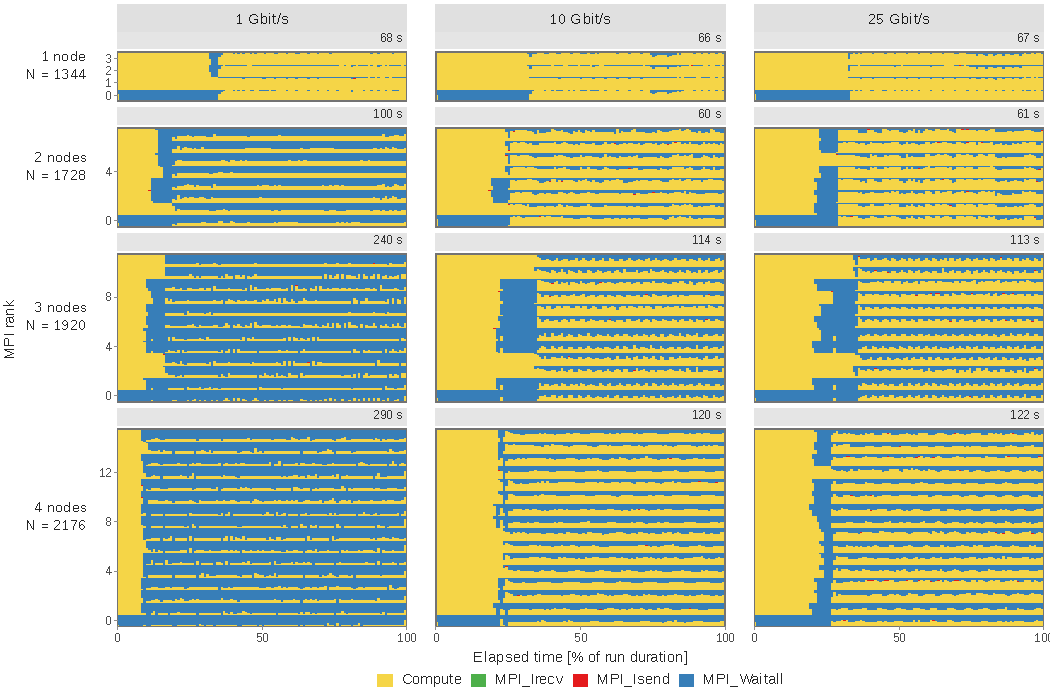
\includegraphics[width=\linewidth]{fig1_masking_timeline_matrix_en.pdf}
  \caption{Temporal composition per rank, by node count and anchor problem size (rows) and bandwidth (columns); median of 5 repetitions.}
  \label{fig:timeline-matrix}
\end{figure}

\subsection{Multi-Node Behavior and Evolution with Scale}

\begin{figure}[tb]
  \centering
  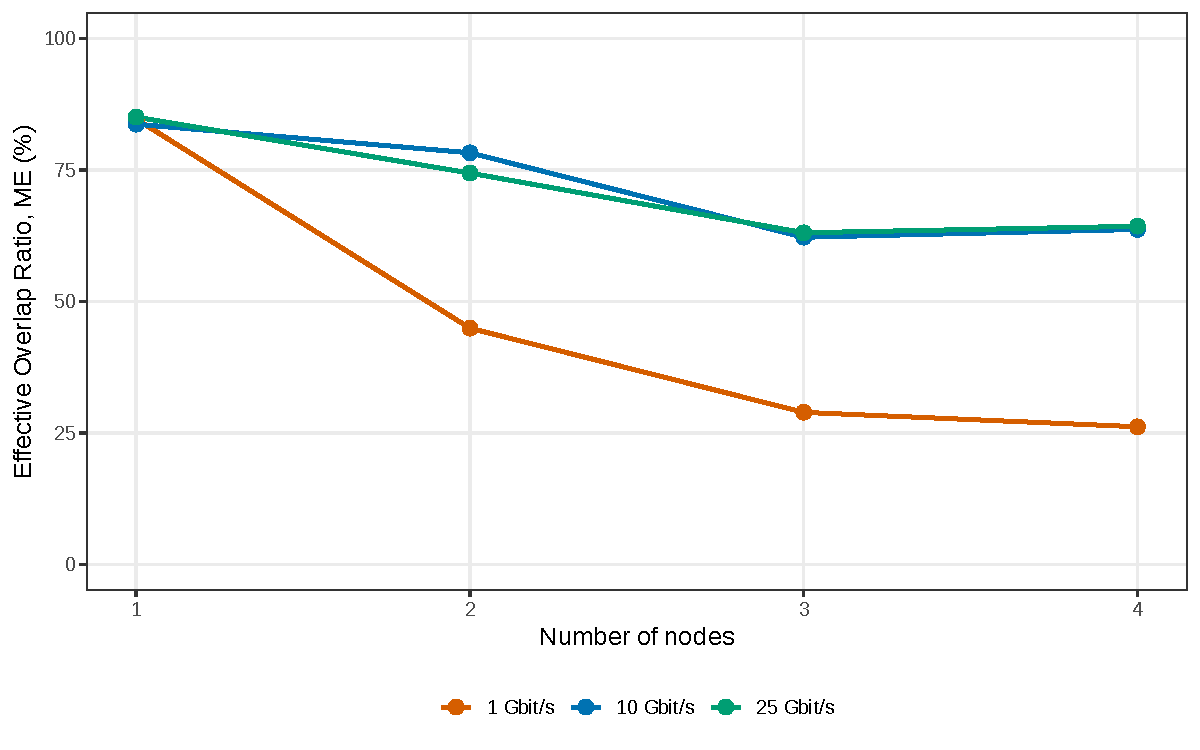
\includegraphics[width=0.72\linewidth]{fig2_masking_effectiveness_vs_nodes_en.pdf}
  \caption{Effective overlap ratio (ME) as a function of node count, for the three bandwidth conditions. Node counts of 1--4 correspond to 4, 8, 12, and 16 A100 GPUs and to anchor sizes $N = 1344/1728/1920/2176$.}
  \label{fig:me-vs-nodes}
\end{figure}

At two nodes (\texttt{2x2x2}, second row of Figure~\ref{fig:timeline-matrix}), ME is 78.3\% at 10~Gbit/s and 74.4\% at 25~Gbit/s, but drops to 44.9\% at 1~Gbit/s, a spread of 33.4 percentage points across bandwidths, beyond what any individual confidence interval would explain (Figure~\ref{fig:me-vs-nodes}). The spread grows to 34.2 percentage points at three nodes (28.9\% against 62.2\%--63.1\%) and 38.2 at four (26.2\% against 63.7\%--64.3\%). The jump occurs upon introducing the first additional node, up from 1.3 percentage point at one node, and subsequent growth is gradual.

Along each row of Figure~\ref{fig:timeline-matrix}, reducing bandwidth from 25 to 1~Gbit/s converts continuous stretches of computation into \texttt{MPI\_Waitall} bands spread across all ranks, an effect absent in the first row and progressively more extensive in the following ones; along each column, increasing the node count widens that waiting fraction even under ample bandwidth, to a lesser degree. The annotated durations quantify the cost in absolute time. The makespan ratio between 1 and 10~Gbit/s goes from 1.03 at one node (68 against 66~s) to 1.67 at two (100 against 60~s), 2.11 at three (240 against 114~s), and 2.42 at four (290 against 120~s), whereas 10 and 25~Gbit/s differ by at most 2~s in any topology.

Figure~\ref{fig:diminishing-returns} compares the two bandwidth transitions available in the campaign, from 1 to 10~Gbit/s and from 10 to 25~Gbit/s, by the ratio between the relative gain of the second and that of the first. The gain from the second transition amounts to roughly 8\% of the first at two nodes, and approaches zero at three and four; the reading holds from two nodes onward, since at one node the gain of the first transition is negligible and the ratio is not physically interpretable. At three nodes, the 0.85 percentage point difference between 10 and 25~Gbit/s is the only one, among the multi-node topologies, that exceeds the corresponding 95\% confidence interval. This pattern of diminishing returns above 10~Gbit/s matches the one projected by the prior study's simulated extension (Section~3.2).

\begin{figure}[tb]
  \centering
  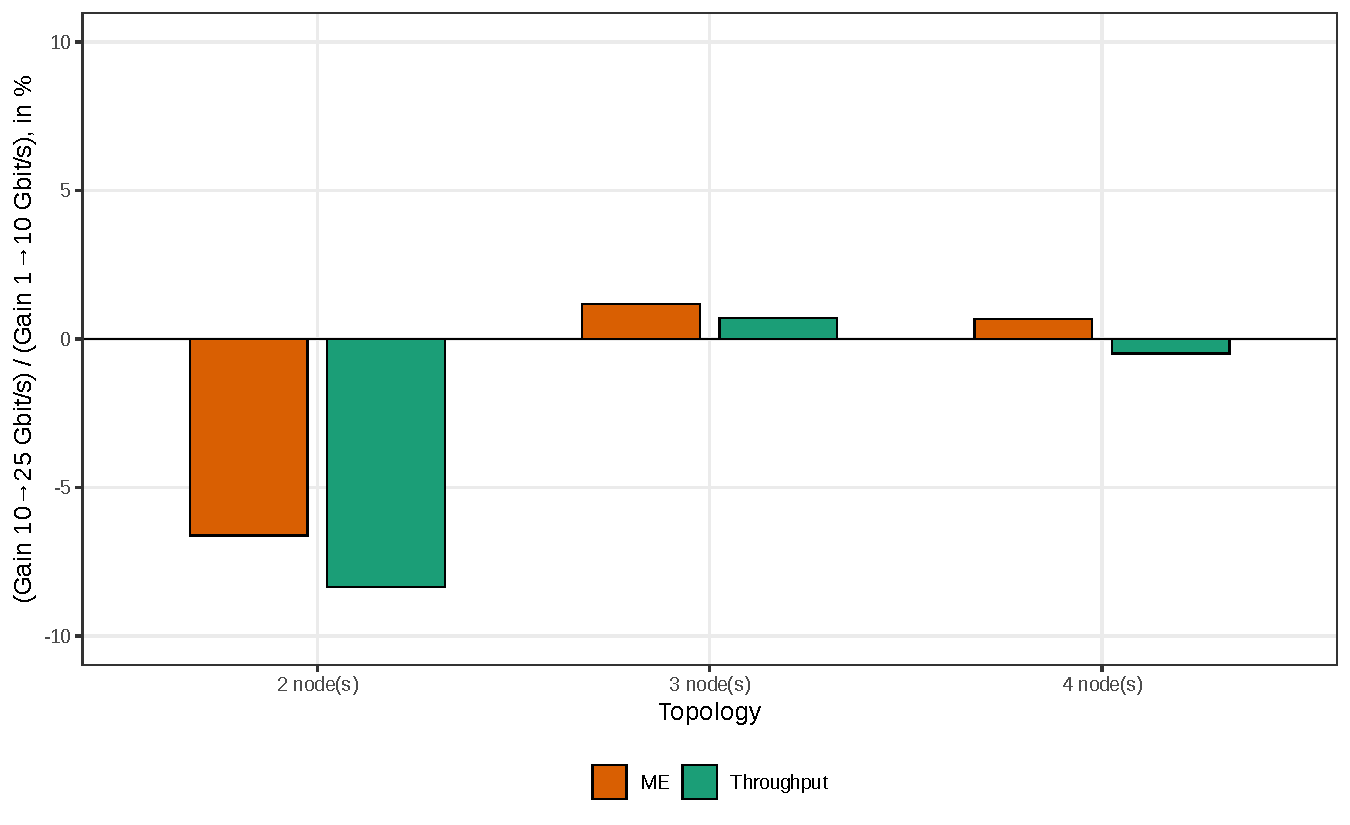
\includegraphics[width=0.72\linewidth]{fig4_diminishing_returns_en.pdf}
  \caption{Ratio between the relative gain of the second bandwidth transition (10$\to$25~Gbit/s) and that of the first (1$\to$10~Gbit/s), per topology, for effective overlap and throughput. A value of 100\% would indicate equal gain in both transitions.}
  \label{fig:diminishing-returns}
\end{figure}

Per-GPU throughput shows that the efficiency loss with scale is not confined to the most constrained bandwidth. At 1~Gbit/s, it falls from 816.6 to 215.4 MSamples/s between one and four nodes, a 73.6\% reduction. At 10 and 25~Gbit/s, the drop is approximately 39\% over the same interval, but it is not monotonic, with a gain when going from one to two nodes ($+17.0$\% and $+12.1$\%), a drop from two to three ($-49.3$\% and $-46.3$\%), and stabilization between three and four. The drop between two and three nodes, present at all three bandwidths, is larger than the remaining transitions. The slope of ME as a function of node count is $-19.2$ percentage points per node at 1~Gbit/s, against $-7.6$ and $-7.4$ at 10 and 25~Gbit/s, with a linear fit of $R^2$ between 0.84 and 0.86, a degradation roughly 2.5 times steeper under constrained bandwidth.

\subsection{Discussion}

\textbf{The predicted direction survives the change of hardware generation.} Under any bandwidth, more nodes reduce ME, and the reduction is sharper the more constrained the bandwidth, consistent with the dependence between communication surface and computational volume on the number of neighbors per process established by \cite{spadotto2026tcc} for block decomposition. In a 3D block decomposition the neighbor count per process is bounded at 26, reached once the grid has at least three subdomains along every axis; growing the node count here still adds neighbors and data exchanged per iteration.

\textbf{Its magnitude does not.} Quantitative validity diverges across bandwidths as scale increases. Under constrained bandwidth, the lengthening of the \texttt{MPI\_Waitall} bands along the first column of Figure~\ref{fig:timeline-matrix} suggests network capacity ceasing to keep up with the volume exchanged per iteration as more processes communicate; above 10~Gbit/s the effect saturates at this scale, indicating bandwidth-insensitive factors this design does not isolate.

\textbf{Part of the cost belongs to scale itself, not to the network.} The per-GPU efficiency drop between two and three nodes persists even under ample bandwidth. One consistent explanation is the change in surface-to-volume ratio when the process grid moves from cubic (\texttt{2x2x2}, two nodes) to non-cubic (\texttt{2x2x3}, three), a dependence discussed in Section~2.1 and not isolated here. The original model, calibrated with one GPU per node and no communication beyond a single neighbor, approximates the direction of the bandwidth effect but not the magnitude of degradation with scale.

\textbf{For dimensioning, extrapolate the direction and measure the magnitude.} For stencil applications distributed across multi-GPU nodes, dimensioning decisions based solely on predictions calibrated at reduced scale tend to underestimate efficiency loss as node count grows, especially under constrained bandwidth; at the tested scales, the return on investing above 10~Gbit/s is limited.

\section{Conclusion}

This work determined the validity envelope of a simulation prediction reused beyond the hardware generation on which it was calibrated. The SimGrid model of Fletcher, calibrated at 1~Gbit/s with one GPU per node \cite{spadotto2026carla}, was confronted with the CUDA backend on the \textit{chuc} cluster of Grid'5000, under three bandwidth conditions and topologies from one to four nodes. The predicted masking trend holds qualitatively beyond the calibration generation, but its quantitative validity depends jointly on bandwidth and scale. The spread in ME across bandwidths grows from 1.3 percentage points at one node to 33.4 at two, 34.2 at three, and 38.2 at four, and the makespan ratio between 1 and 10~Gbit/s goes from 1.03 to 2.42 over the same interval. Above 10~Gbit/s the effect saturates, with an additional gain of roughly 8\% of that obtained in the first transition at two nodes and near zero at three and four; the degradation of ME with scale is $-19.2$ percentage points per node under 1~Gbit/s, against $-7.6$ and $-7.4$ under 10 and 25~Gbit/s, a dependence the original model does not express. For infrastructure dimensioning, the direction of the effect admits extrapolation, whereas its magnitude requires measurement under each configuration of interest. These findings are bounded by the experimental design, a stencil application with block decomposition, a reduced set of problem sizes, and a ceiling of 25~Gbit/s, with GPU generation, network topology, and communication path varying jointly and communication-I/O interaction outside the scope.

Future work includes extending the campaign to larger scales, with process counts that force slices decomposition, to compare the two partitioning topologies on real hardware and confront the factor identified as dominant in the prior study; sweeping problem size per topology to separate the effect of local granularity from that of scale; and recalibrating a platform model for this hardware generation, which would address the fidelity of a new model and extend the envelope delimited here.

\section*{Acknowledgments}

This study was financed in part by the Coordenação de Aperfeiçoamento de Pessoal de Nível Superior (CAPES), Finance Code 001, and by the CNPq/MCTI/FNDCT Universal project no. 408755/2025-3. This work was also partially funded by Petrobras under Agreement no. 4600665938, project GPPD/UFRGS 2.20.2205 (361), Execution of Seismic Applications on Heterogeneous Computing Nodes, EXAFLOP II. The authors thank PCAD/UFRGS for infrastructure access in the prior study's evaluation. Experiments presented in this paper were carried out using the Grid'5000 testbed (specifically the \textit{chuc} cluster), supported by a scientific interest group hosted by Inria and including CNRS, RENATER and several Universities as well as other organizations (see \url{https://www.grid5000.fr}).

{\footnotesize
\let\oldthebibliography\thebibliography
\renewcommand\thebibliography[1]{%
  \oldthebibliography{#1}%
  \setlength{\itemsep}{0pt}%
  \setlength{\parsep}{0pt}%
}
\bibliographystyle{sbc}
\bibliography{referencias}
}

\end{document}